\subsection{Esempi Linguaggi Liberi}
Essendo un linguaggio libero chiuso rispetto alla concatenazione, dati:\\
$L_1 = \{a^nb^nc^j \ / \ n, j \geq 0\} $ Libero\\
$L_2 = \{a^nb^nc^n \ / \ n,j \geq 0\}$ Libero perch\'e concatenazione di $\{a^nb^n\ / \ n \geq 0 \}$ e $\{ c^j \ / \ j \geq 0 \}$, entrambi liberi\\
$L_3 = \{a^nb^nc^n \ / \ n \geq 0\}$ Non \'e libero:

Suppongo $L_3$ libero, sia $p \in \mathbb{N}^+$, $z = a^pb^pc^p$
Allora $z \in  L_3,\ |z|=3p>p$\\
Spacco z in $A=a...a,\ B = b...b, C=c...c$\\
Siano $z = uvwxy\ \land\ |vwx| \leq p \ \land\ |vx| > 0 $:
\begin{itemize}
    \item vwx \'e composto da sole a in A\\
    \item vwx \'e composto da a in A e b in B\\
    \item vwx \'e composto da sole b in B\\
    \item vwx \'e composto da b in B e c in C\\
    \item vwx \'e composto da sole c in C\\
\end{itemize} 
Considero la parola $z' = uv^0wx^0y$ 
\begin{itemize}
    \item[1.] $z' = a^kb^pc^p,\ k<p,\ z' \not\in L_3 $\\
    \item[3.] $z' = a^pb^kc^p,\ k<p,\ z' \not\in L_3 $\\
    \item[5.] $z' = a^pb^pc^k,\ k<p,\ z' \not\in L_3 $\\
    \item[2.] $z' = a^kb^jc^p,\ k<p\ \lor\ j < p ,\ z' \not\in L_3 $\\
    \item[4.] $z' = a^pb^kc^j,\ k<p\ \lor\ j < p ,\ z' \not\in L_3 $\\
\end{itemize}
Quindi visto che la parola non appartiene mai ad $L_3$ il linguaggio non \'e libero.
$\Box$\\[5pt]

\begin{tcolorbox}\begin{center}
    Quindi la classe di linguaggi liberi \textbf{non \'e chiusa rispetto all'intersezione}
\end{center}\end{tcolorbox}

$L_4 = \{a^nb^mc^{n+m} \ / \ n,m>0\}$ Libero\\
$S \rightarrow aSc | aBc$\\
$B \rightarrow bBc|bc$\\

$L_5 = \{ a^nb^mc^nd^m | n,m > 0\}$ Non libero \\
$L_6= \{ wcw^R \ / \ w \in \{a,b\}^+\}$ Libero \\
$S \rightarrow aSa | bSb | aca|bcb$

%%%%%%%%%%%%%%%%%%%%%%%%%%%%%%%%%%%%%%%%%%%%%%%%%%%%%%%%%%%%%%%%%%%%%%%%%%%%%%%%%%%%%%%%%%%%%%%
\chapter{Automi a stati finiti}

Un NFA accetta/riconosce un certo linguaggio.

Sia N un NFA, allora il linguaggio riconosciuto/accettato da N \'e il set delle parole per le quali esiste almeno un cammino dallo stato iniziale di N ad uno stato finale di N.

notare che $\forall\ a \in A,\ a\epsilon = \epsilon a = a$.

%%%%%%%%%%%%%%%%%%%%%%%%%%%%%%%%%%%%%%%%%%%%%%%%%%%%%%%%%%%%%%%%%%%%%%%%%%%%%%%%%%%%%%%%%%%%%%%
\section{Thompson construction}
\begin{center}
    \begin{tabular}{ll}
        input & regular expression r\\
        output & NFA N $\ / \ L(N) = L(r)$\\ 
    \end{tabular}
\end{center}
Gli NFA usati nei passi della costruzione hanno:
\begin{itemize}
    \item un solo stato finale\\ 
    \item non hanno archi entranti sul nodo iniziale\\ 
    \item non hanno archi uscenti dal nodo finale\\
\end{itemize}

\textbf{Lemma}: Lo NFA ottenuto dalle costruzini di Thompson ha al massimo 2k stati e 4k archi, con k lunghezza della re. r.
\textbf{Osservazione}: Ogni passo della costruzione introduce al massimo 2 nodi e 4 archi.

\begin{center}
	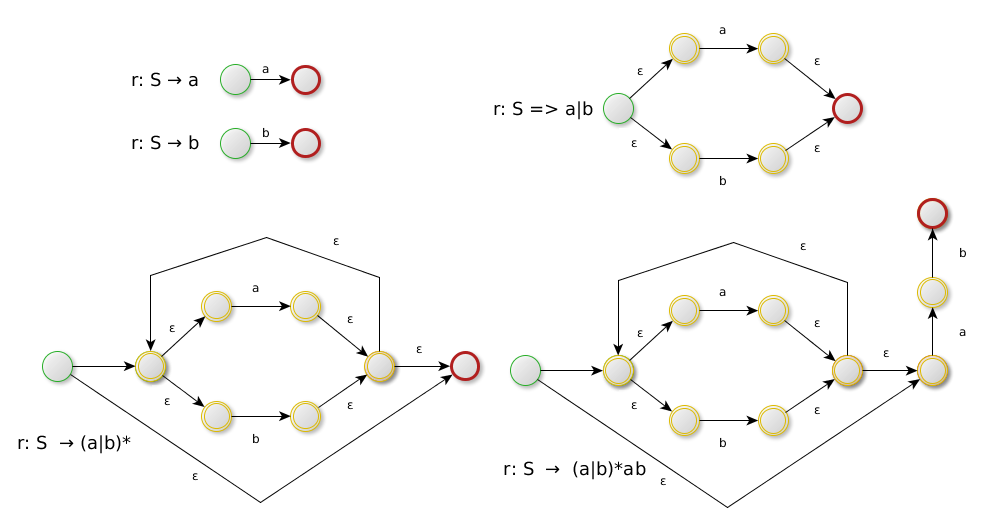
\includegraphics[scale=0.4]{Chapters/Img/c02_01.png}\\
\end{center} 
Algoritmo a complessit\'a $O(|r|)$ 

%%%%%%%%%%%%%%%%%%%%%%%%%%%%%%%%%%%%%%%%%%%%%%%%%%%%%%%%%%%%%%%%%%%%%%%%%%%%%%%%%%%%%%%%%%%%%%%
\section{Simulare un NFA}
Il backtracking consiste nel seguire un percorso e se non va bene tornare in dietro e provarne un altro finch\'e alla fine 
li provo tutti mal che vada.

$N=(S,A,move_n,S_0,F)$, S insieme stati, A degli archi, $S_0$ stato iniziale, F set stati finali, $move_n$ funzione di transizione\\
$t \in S, T \subset S$\\
$\epsilon - closure(\{ t \})$ il set degli stati S raggiungibili tramite \underline{zero o pi\'u} 
$\epsilon -transizioni$ da t (in pratica il nodo stesso e tutti i nodi raggiungibili con una $\epsilon-transition$).

Nota che $\forall t \in S,\ t\in \epsilon-closure(t)$\\
$\epsilon-closure(T) = \cup _{t \in T} \epsilon-closure(t)$

Questo algoritmo \'e pi\'u performante del backtracking.

%%%%%%%%%%%%%%%%%%%%%%%%%%%%%%%%%%%%%%%%%%%%%%%%%%%%%%%%%%%%%%%%%%%%%%%%%%%%%%%%%%%%%%%%%%%%%%%
\subsection{Algoritmo per la computazione}
Strutture dati:
\begin{itemize}
    \item pila\\
    \item bool[] alreadyOn, dimensione $|S|$\\
    \item array[][] $move_n$\\ 
\end{itemize}
\begin{lstlisting}
    for(int i = 0; i < |S|; i++){
        alreadyOn[i] = false;
    }
    closure(t, stack){
        push t onto stack;
        alreadyOn[t] = true; //posso sempre arrivare a me stesso con una epsilon-transition 
        foreach(i in move_n(t, epsilon)){
            if(!alreadyOn[i]){
                closure(i, stack);
            }
        }
    }
\end{lstlisting}

\begin{center}
	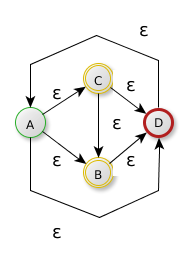
\includegraphics[scale=0.4]{Chapters/Img/c02_02.png}\\
\end{center} 

\begin{lstlisting}
    alredyOn[F F F F];
    closure(A, pila vuota)
        [A] [T F F F]
            //B non e' ancora nella pila
            closure(B, [A])
                [A, B] [T T F T]
                closure(D, [A, B])
                    [A, B, D] [T T F T]
            closure(C, [A, B, D])
                [A, B, C, D] [T T T T]
\end{lstlisting}

%%%%%%%%%%%%%%%%%%%%%%%%%%%%%%%%%%%%%%%%%%%%%%%%%%%%%%%%%%%%%%%%%%%%%%%%%%%%%%%%%%%%%%%%%%%%%%%
\subsection{Algoritmo per la simulazione di un NFA}
\begin{center}
    \begin{tabular}{ll}
        input & NFA N, w$\$$\\
        output & yes se $w \in L(N)$, no altrimenti\\ 
    \end{tabular}
\end{center}
\begin{lstlisting}
    N = (S, A, move_n, S_0, F)
    states = epsilon-closure({S_0})
    symbol = nextchar()
    while(symbol != $){
        states = epsilon-closure(Unione_{t in states} di move_n(t, symbol));
        symbol = newxtchar();
    }
    if(states intersecato F != emptyset){
        return yes;
    }
    return no;
\end{lstlisting}

%TODO GRAFO PAGINA 17

Algoritmo a complessit\'a $O(|w|(n+m))$ 


%%%%%%%%%%%%%%%%%%%%%%%%%%%%%%%%%%%%%%%%%%%%%%%%%%%%%%%%%%%%%%%%%%%%%%%%%%%%%%%%%%%%%%%%%%%%%%%
\section{DFA}
Automa a stati finiti, deterministico; una sottoclasse degli NFA che rispettano:
\begin{center}
    DFA$\overset{\Delta}{=}(S,A,move_d,s_0,F)$  \\
    $move_d \overset{\Delta}{=} (S \otimes A) \rightarrow S$\\
\end{center}
\begin{itemize}
    \item non hanno $\epsilon-transizioni$\\
    \item $\forall a \in A, s \in S,\ move_n(s,a)$ \'e un unico stato se \textbf{funzione di transizione totale} 
    (al pi\'u uno stato se \textbf{funzione di transizione parziale})\\
\end{itemize}
\begin{tcolorbox}\begin{center}
    Sink è il nodo pozzo dove confluiscono tutte le transizioni non segnate;
    viene aggiunto per rendere la funzione di transizione una funzione di transizione totale
\end{center}\end{tcolorbox}

%%%%%%%%%%%%%%%%%%%%%%%%%%%%%%%%%%%%%%%%%%%%%%%%%%%%%%%%%%%%%%%%%%%%%%%%%%%%%%%%%%%%%%%%%%%%%%
\subsection{Linguaggio riconosciuto dal DFA}
Dato il DFA D, L(D) \'e il linguaggio riconosciuto da D. \\
$L(D) = \{ w=a_1,...,a_k \ / \ \exists \text{ cammino in D dallo stato iniziale al finale}\}$.
$\epsilon \in L(D) \iff s_0 \in F$.

\subsection{Simulazione di un DFA con $move_d$ totale}
\begin{center}
    \begin{tabular}{ll}
        input & w$\$$, DFA $D=(S,A,move_d,F)$\\
        output & yes se $w \in L(D)$, no altrimenti\\
    \end{tabular}
\end{center}

\begin{lstlisting}
    state = s_0;
    while(symbol != $ && state != bottom){
        //move_d(s, a) = bottom <=> move_d non e' definita su (s,a)
        state = move_d(state, symbol);
        symbol = newxtchar();
    }
    if(state \in F)
        return yes;
    return true;
\end{lstlisting}

Simulazione NFA costa $O(|w|(n+m))$
Simulazione DFA costa $O(|w|)$

\section{Subset Construction}
\begin{center}
    \begin{tabular}{ll}
        input & $NFA(S^n,A,move_n, S_0 ^n,F^n)$\\ 
        output & $DFA(S^d,A,move_d, S_0 ^d,F^d)$\\
    \end{tabular}
\end{center}

\begin{lstlisting}
    
\end{lstlisting}